%%%%%%%%%%%%%%%%%%%%%%%%%%%%%%%%%%%%%%%%%
% Preliminary
%
% In this section, I will briefly discuss conditional flow-matching and Mean Flows for one-step generation
%
\section{Preliminaries}
\label{sec: preliminary}

\noindent\textbf{Flow-Matching.} Let $\vx$ denote a data sample in $\gX\subset\mathbb{R}^{d}$ . Flow-matching generative models~\cite{lipman2023flowmatchinggenerativemodeling,tong2024improvinggeneralizingflowbasedgenerative} learn a time-dependent diffeomorphism $\psi(\vx,t):\mathbb{R}^{d}\!\times\![0,1]\to\mathbb{R}^{d}$ from a simple distribution $\rvx_{1}\!\sim\!{p}(\rvx,1)$ to the target $\rvx_{0}\!\sim\!{p}(\rvx,0)\!=\!\pdata$ by parameterizing a velocity field $\vv(\vx,t)\!\triangleq\!\frac{\mathrm{d}}{\mathrm{d}t}\psi(\vx,t)$. Since the exact \textit{marginal velocity field} $\vv(\vx,t)$ is generally inaccessible, conditional flow-matching~\cite{lipman2023flowmatchinggenerativemodeling} instead learns a conditional field $\vv_{\text{cond}}\!=\!\vx_{1}-\vx_{0}$ with $\vx_{t}\!=\!(1-t)\vx_{0}+t\vx_{1}$. The following lemma justifies the substitution. See~\Cref{appx: first} for its proof.
\begin{lemma}
    Given vector fields $\vv_{\text{cond}}$ generating conditional probability paths $p(\vx,t\mid\vx_{0})$, for any $\rvx_{0}\!\sim\!p(\rvx_{0})$, the expected conditional velocity field is equal to the marginal velocity field
    \begin{equation}
        \vv(\vx,t)=\E_{\vx_{0}\sim{p(\vx_{0}\mid\vx_{t}=\vx)}}\!\left[\vv(\vx,t\mid\vx_{0})\right].
        \label{eq: margv-condv-relation}
    \end{equation}
\end{lemma}

%%%%%%%%%%%%%%%%%%%%%%%%%%%%%%%%%%%%%%%%%
% MeanFlow
%%%%%%%%%%%%%%%%%%%%%%%%%%%%%%%%%%%%%%%%%
\noindent\textbf{One-step Mean Flows.} Iterative integration of $\vv(\vx,t)$ at inference is expensive and can be numerically unstable. To bypass it, Mean Flows~\cite{geng2025meanflowsonestepgenerative} learn a two-parameter average velocity field $\vu(\rvx,r,t)$ through regressing an identity along the flow trajectory $\vx_{\tau}\!=\!\psi(\vx_{r},\tau)$ with terminal at $\vx_{t}\!=\!\vx$:
\begin{equation}
    (t-r)\,\vu(\vx,r,t)=\int_{r}^{t}\vv(\vx_{\tau},\tau)\,\mathrm{d}\tau.
    \label{eq: meanflow-identity}
\end{equation}
Differentiating with respect to the terminal time $t$ along the same trajectory yields
\begin{equation}
    \vu(\vx,r,t)+(t-r)\tfrac{\mathrm{d}}{\mathrm{d}t}\vu(\vx,r,t)=\vv(\vx,t),\qquad
    \tfrac{\mathrm{d}}{\mathrm{d}t}\vu=\partial_{\vx}\vu\!\cdot\!\vv(\vx,t)+\partial_{t}\vu,
    \label{eq: td-meanflow-identity}
\end{equation}
where the total derivative $\frac{\mathrm{d}}{\mathrm{d}t}\vu$ is essentially a JVP, denoted by $\texttt{JVP}(\vu,(\vx,r,t),(\vv(\vx,t),0,1))$. The original MeanFlow paper~\cite{geng2025meanflowsonestepgenerative} replaces \emph{both} occurrences of the marginal field with the conditional field $\vv_{\text{cond}}\!=\!\vx_{1}\!-\!\vx_{0}$, giving the MeanFlow loss
\begin{equation}
    \mathcal{L}_{\text{MF}}(\vtheta)=
    \E_{r,t,\vx_{0},\vx_{1}}\!\left[\left\|\vu_{\vtheta}+(t-r)\,\texttt{sg}\!\left[\texttt{JVP}(\vu_{\vtheta},(\vx_{t},r,t),(\vv_{\text{cond}},0,1))\right]-\vv_{\text{cond}}\right\|_{2}^{2}\right],
    \label{eq: mf-loss}
\end{equation}
with $r,t\!\sim\!\gU(0,1)$, $r\!\leq\!t$, $\vx_{0}\!\sim\!\pdata$, $\vx_{1}\!\sim\!\gN(0,\mI_{d})$, $\vx_{t}\!=\!(1-t)\vx_{0}+t\vx_{1}$, and the stop-gradient $\texttt{sg}[\cdot]$ avoiding double backpropagation through the JVP.

%%%%%%%%%%%%%%%%%%%%%%%%%%%%%%%%%%%%%%%%%%%%%%%%%%%%%%%%%%%%%%%%%%%%%%%%%%%%%%%%
% Variance Reduction in Learning Mean Flows
%%%%%%%%%%%%%%%%%%%%%%%%%%%%%%%%%%%%%%%%%%%%%%%%%%%%%%%%%%%%%%%%%%%%%%%%%%%%%%%%
\section{Variance Reduction in Learning Mean Flows}
\label{sec: method}

The MeanFlow loss in~\eqref{eq: mf-loss} is empirically known to be \textit{non-decreasing} and to suffer from \textit{high-variance gradients}~\cite{zhang2025alphaflowunderstandingimprovingmeanflow,geng2025improvedmeanflowschallenges}. We investigate the statistical mechanism behind this pathology. Importantly, our analysis isolates the role of the conditional velocity field $\vv_{\text{cond}}$ when it appears as the JVP tangent, and identifies that it acts as a Monte Carlo control variate for the inaccessible marginal velocity, with a coefficient that the original MeanFlow fixes to a suboptimal value. We derive the optimal coefficient and establish a connection to practical fixes in concurrent works.

%%%%%%%%%%%%%%%%%%%%%%%%%%%%%%%%%%%%%%%%%
\subsection{Two roles of the conditional velocity field}
\label{subsec: two-roles}

With Reynolds decomposition, we express the conditional velocity by $\vv_{\text{cond}}\!=\!\vv(\vx,t)+\vv^{\prime}$ with $\E_{\vx_{0}\mid\vx_{t}}[\vv^{\prime}]\!=\!\bm{0}$ according to~\eqref{eq: margv-condv-relation} and $\Sigma_{\vv^{\prime}}\!\triangleq\!\Cov_{\vx_{0}\mid\vx_{t}}[\vv^{\prime}]$. The MeanFlow loss in~\eqref{eq: mf-loss} uses $\vv_{\text{cond}}$ both as the \textit{regression target} and as the \textit{tangent} inside the total derivative. Carrying the decomposition through per-sample loss $\ell_{\text{MF}}(\vtheta)$ yields:
\begin{equation}
    \E_{\vx_{0}\mid\vx_{t}}\!\bigl[\ell_{\text{MF}}(\vtheta)\bigr]
    =\bigl\|\vr_{\vtheta}^{\texttt{sg}}\bigr\|^{2}_{2}
    +\texttt{sg}\!\bigl[\Tr(\mJ\Sigma_{\vv^{\prime}}\mJ^{\!\top})\bigr],
    \label{eq: per-sample-expand}
\end{equation}
where $\mJ\!\triangleq\!(t{-}r)\partial_{\vx_{t}}\vu_{\vtheta}\!-\!\mI_{d}\!\in\!\mathbb{R}^{d\times d}$ is a \textit{Jacobi factor} determined by the Jacobian matrix $\partial_{\vx_{t}}\vu_{\vtheta}$ and $\vr_{\vtheta}^{\texttt{sg}}\!\triangleq\!\vu_{\vtheta}\!+\!(t{-}r)\,\texttt{sg}[\partial_{\vx_{t}}\vu_{\vtheta}\!\cdot\!\vv\!+\!\partial_{t}\vu_{\vtheta}]\!-\!\vv$ is the deterministic mean-field residual. Since the residual $\vr_{\vtheta}^{\texttt{sg}}$ is the exact loss we aim to minimize given by~\eqref{eq: td-meanflow-identity}, the trace term leads to the non-decreasing loss and eliminates $\textit{iff}$ the Jacobi satisfies $\partial_{\vx_{t}}\vu_{\vtheta}=\frac{1}{t-r}\mI_{d}$ (equivalently, $\mJ\!=\!\bm{0}$). We identify two roles of the conditional velocity field in this decomposition:

\noindent\textbf{Unbiased Target.} As the regression target, $\vv_{\text{cond}}$ injects $\vv^{\prime}$ \textit{linearly} into the residual, contributing the \emph{irreducible} per-sample noise floor $\Tr(\Sigma_{\vv^{\prime}})$. However, since this noise is independent of $\vtheta$ and $\vv^{\prime}$ is zero-mean, $\vv_{\text{cond}}$ can serve as an unbiased target for learning Mean Flows.

\noindent\textbf{Variance Amplifier.} As the JVP tangent, the same $\vv_{\text{cond}}$ injects $\vv^{\prime}$ \textit{multiplicatively} through the Jacobi factor $\mJ$, contributing the \emph{amplified} term $\Tr(\mJ\Sigma_{\vv^{\prime}}\mJ^{\!\top})$. It scales unboundedly with the spectral magnitude of $\mJ$. This amplification is the dominant driver of variance at the gradient level:

\begin{theorem}[Jacobian Variance Amplification]
    Let $\vg\!\triangleq\!\nabla_{\vtheta}\vu_{\vtheta}(\vx_{t},r,t)\!\in\!\mathbb{R}^{d\times p}$ be the parameter Jacobian of the average velocity. The trace of the conditional gradient covariance (\textit{i.e., the total variance}) of $\ell_{\text{MF}}(\vtheta)$ in~\eqref{eq: mf-loss} satisfies
    \begin{equation*}
        \boxed{
            \Tr\!\left(\Cov\!\left[\nabla_{\vtheta}\ell_{\text{MF}}\mid\vx_{t}\right]\right)
            \;\propto\;
            \Tr\!\left(\vg^{\!\top}\,\mJ\,\Sigma_{\vv^{\prime}}\,\mJ^{\!\top}\,\vg\right).
        }
    \end{equation*}
    \label[theorem]{thm: jacobi-variance}
\end{theorem}

See the proof in~\Cref{appx: theorem-proof}. The theorem identifies that the total gradient variance grows with $\|\mJ\|^{2}$ for fixed $\vg$ and $\Sigma_{\vv^{\prime}}$, saturates only at the irreducible noise floor when $\mJ\!\to\!\bm{0}$, and is \emph{uncontrolled} by any term in the loss due to the use of the stop-gradient in the original MeanFlow. Meanwhile, without the stop-gradient operator, the optimizer could in principle reduce variance by driving $\mJ\!\to\!\bm{0}$. This establishes a \textit{semi-gradient gap}, formally,

\begin{theorem}[Semi-Gradient Gap]
    The gradient of the MeanFlow loss $\gL_{\text{MF}}$ with and without the stop-gradient operator differ by
    \begin{equation}
        \boxed{
            \underbrace{2(t{-}r)\,\E\!\left[\bigl(\nabla_{\vtheta}\!\left(\partial_{\vx_{t}}\vu_{\vtheta}\!\cdot\!\vv+\partial_{t}\vu_{\vtheta}\right)\bigr)^{\!\top}\vr_{\vtheta}\right]}_{\text{mean-field gradient difference}}
            +\underbrace{\E\!\left[\nabla_{\vtheta}\Tr\!\left(\mJ\Sigma_{\vv^{\prime}}\mJ^{\!\top}\right)\right]}_{\text{variance-driven gradient difference}}.
        }
    \end{equation}
    \label[theorem]{thm: semi-gradient-gap}
\end{theorem}

In the original MeanFlow, the stop-gradient operator prevents $\mJ$ from being passed to the optimizer, leading to an empirical non-decreasing loss. Meanwhile, the mean-field difference vanishes at convergence ($\vr_{\vtheta}\!\to\!\bm{0}$) and the variance-driven term $\Tr(\mJ\Sigma_{\vv^{\prime}}\mJ^{\!\top})$ dominates. To better illustrate the idea, \Cref{fig: cm-gap} visualizes the spatial distribution of $\sqrt{\E_{\vx_{0}\mid{\vx_{t}}}\left\|\vv^{\prime}\right\|^{2}}$ on a three-mode, two-dimensional Gaussian mixture. It showcases that the total variance magnitude is non-zero, concentrates in mode-mixing regions where conditional paths overlap, and grows toward the latent endpoint ($t\!\to\!1$).

\begin{figure}[t]
    \centering
    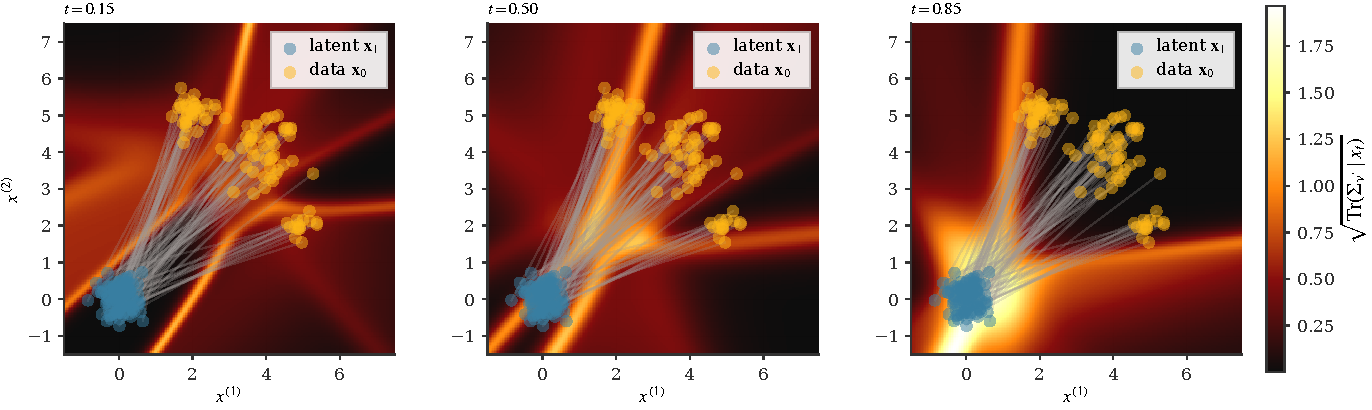
\includegraphics[width=\textwidth]{assets/figures/illustration.pdf}
    \caption{Spatial distribution of $\sqrt{\Tr(\Sigma_{\vv^{\prime}}\!\mid\!\vx_{t})}\!=\!\sqrt{\E_{\vx_{0}\mid\vx_{t}}\|\vv^{\prime}\|^{2}}$ at three timesteps on a two-dimensional Gaussian mixture. Conditional variances concentrate in mode-mixing regions.}
    \label{fig: cm-gap}
    \vspace{-1em}
\end{figure}

%%%%%%%%%%%%%%%%%%%%%%%%%%%%%%%%%%%%%%%%%
\subsection{Rethinking tangent as a control variate}
\label{subsec: control-variate}

The amplification in~\Cref{thm: jacobi-variance} arises due to using $\vv_{\text{cond}}\!=\!\vv\!+\!\vv^{\prime}$ as the JVP tangent injects the zero-mean fluctuation $\vv^{\prime}$. Hence, $\vv_{\text{cond}}$ is analogous to the canonical structure of a Monte Carlo \textit{control variate}~\cite{glasserman2003montecarlo}, where $\vv_{\text{cond}}$ is a stochastic estimator of the inaccessible $\vv$ with known mean, and the coefficient on the noise term $\vv^{\prime}$ determines the bias-variance trade-off. To make this explicit, we introduce a tangent-mixing coefficient $\beta\!\in\![0,1]$:
\begin{equation}
    \tilde{\vv}_{\text{tang}}(\beta)\;\triangleq\;(1-\beta)\,\vv_{\text{cond}} + \beta\,\hat{\vv}\;=\;\vv + (1-\beta)\,\vv^{\prime} + \beta\,\vb,
    \label{eq: tangent-mix}
\end{equation}
where $\hat{\vv}$ can be any deterministic proxy for the marginal velocity (\textit{e.g., a velocity network}) with bias $\vb\!\triangleq\!\hat{\vv}-\vv$ that is deterministic given $\vx_{t}$. Herein, $\beta\!=\!0$ recovers vanilla MeanFlow and $\beta\!=\!1$ replaces the tangent entirely with the deterministic proxy.

\noindent\textbf{Bias-variance trade-off.} Substituting $\tilde{\vv}_{\text{tang}}(\beta)$ for $\vv_{\text{cond}}$ in the JVP tangent and propagating through the loss, the per-sample gradient writes
\begin{equation}
    \vg^{(\beta)} \;=\; 2\,\vg^{\!\top}\!\Bigl[\vr_{\vtheta} \;+\; \bigl((1{-}\beta)\,\mJ - \beta\,\mI\bigr)\,\vv^{\prime} \;+\; \beta\,(\mJ{+}\mI)\,\vb\Bigr],
    \label{eq: g-beta}
\end{equation}
where the noise term scales the conditional fluctuation $\vv^{\prime}$ by the matrix $((1{-}\beta)\,\mJ - \beta\,\mI)$, and the bias term scales the proxy error $\vb$ by $\beta\,(\mJ{+}\mI)$. In this case, we can balance the bias-variance trade-off through solving for the optimal coefficient $\beta^{\ast}$ that minimizes the least-squares between the expected per-sample gradient in~\eqref{eq: g-beta} and the target gradients, given by
\begin{equation}
    M(\beta)\;\triangleq\;\E_{\vv^{\prime}\mid{\vx_{t}}}\left[\left\|\vg^{(\beta)}-\nabla_{\vtheta}\|\vr_{\vtheta}\|_{2}^{2}\right\|_{2}^{2}\right]\;=\;\E_{\vv^{\prime}\mid{\vx_{t}}}\left[\left\|\vg^{(\beta)}-2\vg^{\top}\vr_{\vtheta}\right\|_{2}^{2}\right].
    \label{eq: beta-target}
\end{equation}
We derive the following theorem.

\begin{theorem}[Optimal control-variate coefficient]
    Under the scalar-isotropic approximation $\Sigma_{\vv^{\prime}}\!\approx\!\sigma^{2}\mI_{d}$, $\mJ\!\approx\!\kappa\mI_{d}$, and the parameter-isotropy approximation $\vg\vg^{\!\top}\!\propto\!\mI_{d}$ (which reduces $M$ to a per-component MSE; cf.~\Cref{appx: theorem-proof}),
    \begin{equation*}
        M(\beta) \;\propto\; \beta^{2}(\kappa{+}1)^{2}\|\vb\|^{2} + \sigma^{2}d\bigl((1{-}\beta)\kappa - \beta\bigr)^{2}.
    \end{equation*}
    For $\kappa\!>\!0$, $M(\beta)$ admits a unique minimizer
    \begin{equation}
        \boxed{
            \beta^{\ast} \;=\; \underbrace{\frac{\kappa}{\kappa+1}}_{\text{noise-cancellation}}\;\cdot\;\underbrace{\frac{\sigma^{2}d}{\sigma^{2}d + \|\vb\|^{2}}}_{\text{shrinkage}},
        }
        \label{eq: beta-minimizer}
    \end{equation}
    with optimum value $M(\beta^{\ast})\!\propto\!\sigma^{2}d\,\kappa^{2}\,\|\vb\|^{2}/(\sigma^{2}d+\|\vb\|^{2})$.
    % For all $\kappa,\|\vb\|^{2}\!>\!0$, $M(\beta^{\ast})$ strictly dominates both corner MSEs $M(0)\!\propto\!\sigma^{2}\kappa^{2}d$ (vanilla MeanFlow) and $M(1)\!\propto\!(\kappa{+}1)^{2}\|\vb\|^{2}+\sigma^{2}d$ (deterministic-tangent estimator with bias). The boundary case $\kappa\!=\!-1$ (which corresponds to $\partial_{\vx_{t}}\vu_{\vtheta}\!=\!\bm{0}$ at initialization) leaves $M(\beta)$ constant and is excluded.
    \label[theorem]{thm: control-variate-optimum}
\end{theorem}

See the proof in~\Cref{appx: theorem-proof}. The two components of $\beta^{\ast}$ play distinct roles: $\kappa/(\kappa{+}1)$ is the coefficient that \emph{cancels the Jacobian-amplified noise} through destructive interference between the $\mJ\vv^{\prime}$ and $\mI\vv^{\prime}$ contributions in~\eqref{eq: g-beta}, while $\sigma^{2}d/(\sigma^{2}d{+}\|\vb\|^{2})$ is the standard James-Stein shrinkage~\cite{james1961estimation} that pulls $\beta^{\ast}$ toward the unbiased corner when the proxy bias $\|\vb\|$ is large. Therefore, as the proxy bias shrinks ($\|\vb\|^{2}\!\to\!0$), $\beta^{\ast}\!\to\!\kappa/(\kappa{+}1)$, and as the Jacobian magnitude grows ($\kappa\!\to\!\infty$), $\beta^{\ast}\!\to\!1$. Following the theory, we explain the high variance of gradients in the original MeanFlow and establish a connection to practical fixes in concurrent work.

\noindent\textbf{High-variance gradient with suboptimal coefficient.} The original MeanFlow uses $\beta\!=\!0$ which is optimal only when $\kappa\!=\!0$ (i.e., $\partial_{\vx_{t}}\vu_{\vtheta}\!=\!\frac{1}{t-r}\mI_{d}$) or when no deterministic proxy is available ($\|\vb\|\!=\!\infty$). Both conditions fail in practice: trained backbones produce $\partial_{\vx_{t}}\vu_{\vtheta}$ matrices that are spectrally far from $\frac{1}{t-r}\mI_{d}$, and there are multiple viable deterministic proxies for the marginal $\vv$.

\begin{table}[t]
    \centering
    \small
    \caption{Concurrent MeanFlow remedies positioned in our control-variate framework. Each method either drives $\beta\!\to\!1$ with a deterministic proxy, reduces the amplification factor $\|\mJ\|^{2}$ directly, or replaces the JVP construction altogether.}
    \label{tab: concurrent-positioning}
    \begin{tabular}{@{}lll@{}}
        \toprule
        Method & Mechanism in our framework & Practical realization \\
        \midrule
        AlphaFlow~\cite{zhang2025alphaflowunderstandingimprovingmeanflow} & avoid high-$\kappa$ regimes & $\alpha$-curriculum schedule \\
        Improved MF~\cite{geng2025improvedmeanflowschallenges} & deterministic tangent ($\beta\!\to\!1$) & separate velocity head + sg \\
        Modular MF~\cite{you2025modularmeanflow} & deterministic tangent ($\beta\!\to\!1$) & gradient-modulated loss family \\
        Kim~\textit{et al.}~\cite{kim2025understandingacceleratingmeanflow} & deterministic tangent ($\beta\!\to\!1$) & staged training schedule \\
        TVM~\cite{zhou2026terminalvelocitymatching} & remove the spatial Jacobian ($\mJ\!\to\!\bm{0}$) & terminal-time differentiation \\
        Re-MeanFlow~\cite{zhang2026overcomingcurvaturebottleneckmeanflow} & reduce $\|\mJ\|$ & rectified-flow preprocessing \\
        Rectified MF~\cite{zhang2025rectifiedmeanflow} & reduce $\|\mJ\|$ & self-distilled trajectory straightening \\
        Decoupled MF~\cite{lee2025decoupledmeanflow} & bypass JVP construction & flow-map conditioning on later $t$ \\
        \textbf{VaMF (ours)} & deterministic tangent ($\beta\!\to\!1$) & EMA proxy + FM anchor \\
        \bottomrule
    \end{tabular}
\end{table}


\noindent\textbf{Concurrent works as control variates.} Our theory unifies several remedies for MeanFlow's training pathology across concurrent works into a single one-parameter family. Each empirical fix corresponds to a different practical realization of the optimum $\beta^{\ast}$, distinguished by \emph{which proxy} they use for $\vv$ and \emph{which value of $\beta$} the construction implicitly selects. We summarize them in~\cref{tab: concurrent-positioning}.
